\documentclass[10pt, a4paper]{article}
\usepackage[top=0.6in,bottom=1.0in,left=1.0in,right=1.0in]{geometry}
\usepackage{amsmath,amssymb}
\usepackage{hyperref}
\fontfamily{times}
\usepackage{graphicx,float,tikz}

\title{\large CS 4366: Senior Capstone Project \\ Dr. Sunho Lim \\ Project \#3 - Software Design Specification - Project Report \\ EmergenSeek}
\author{Suhas Bacchu \ Derek Fritz \ Kevon Manahan \ Annie Vo \ Simon Woldemichael}
\date{February 27, 2019}

\begin{document}

\maketitle
\vspace{-1cm}
\begin{abstract}
In this report, we describe and detail the layout and design of EmergenSeek. The structure of the system, at a high-level, consists of two components; a mobile client, developed using a Dart-based, cross-platform mobile framework called Flutter, and a backend API, developed using Amazon Web Services and the Go programming language. Each of these components is also broken down into their own modules and components. Respective design documentation, including UML class, use case, and sequence diagrams, are included as well.
\end{abstract}

\section{Design Documentation}
\par ~ In this section, we will discuss the various details of our design documents.

\subsection{UML Class Diagram}
\subsection{UML Use-case Diagram}
\subsection{UML Sequence Diagrams}

\section{Client Analysis}
\par ~ In this section, we will enumerate the various modules and components responsible for keeping the frontend functional.

\section{Backend Analysis}
\par ~ In this section, we will enumerate the various modules, components, and objects responsible for keeping the backend functional. It should be noted that there is no literal \texttt{class} instance within the Go programming language, but objects may still be enumerated through the \texttt{struct} qualifier. Class attributes are defined as \texttt{struct} fields.

\subsection{Models}
\par ~ The models of this application contain Go structures which replicate 

\subsection{Subsystems}
\par ~ The backend of the application will utilize AWS Lambda, a serverless, Functions-as-a-Service offering to run our Go code, DynamoDB to store user data and information, the Twilio API to provide the system with programmable SMS and voice communications, and Google's Geocoding and Maps APIs to better define the location of users and various emergency services. The subsystems of the application are divided up into single-responsibility, service-oriented architecture. This means that the backend consists of several Lambda functions and each function is responsible for only one thing. In total, at the time of this report, there are \emph{six} Lambda functions. Here is a breakdown of their functionality. Functions are prefixed with \texttt{ES} and suffixed with a meaningful name which explains their role.

\subsubsection{Lambda Function 1}
\subsubsection{Lambda Function 2}
\subsubsection{Lambda Function 3}
\subsubsection{Lambda Function 4}
\subsubsection{Lambda Function 5}
\subsubsection{Lambda Function 6}

\begin{figure}[H]
\begin{center}
\centerline{
	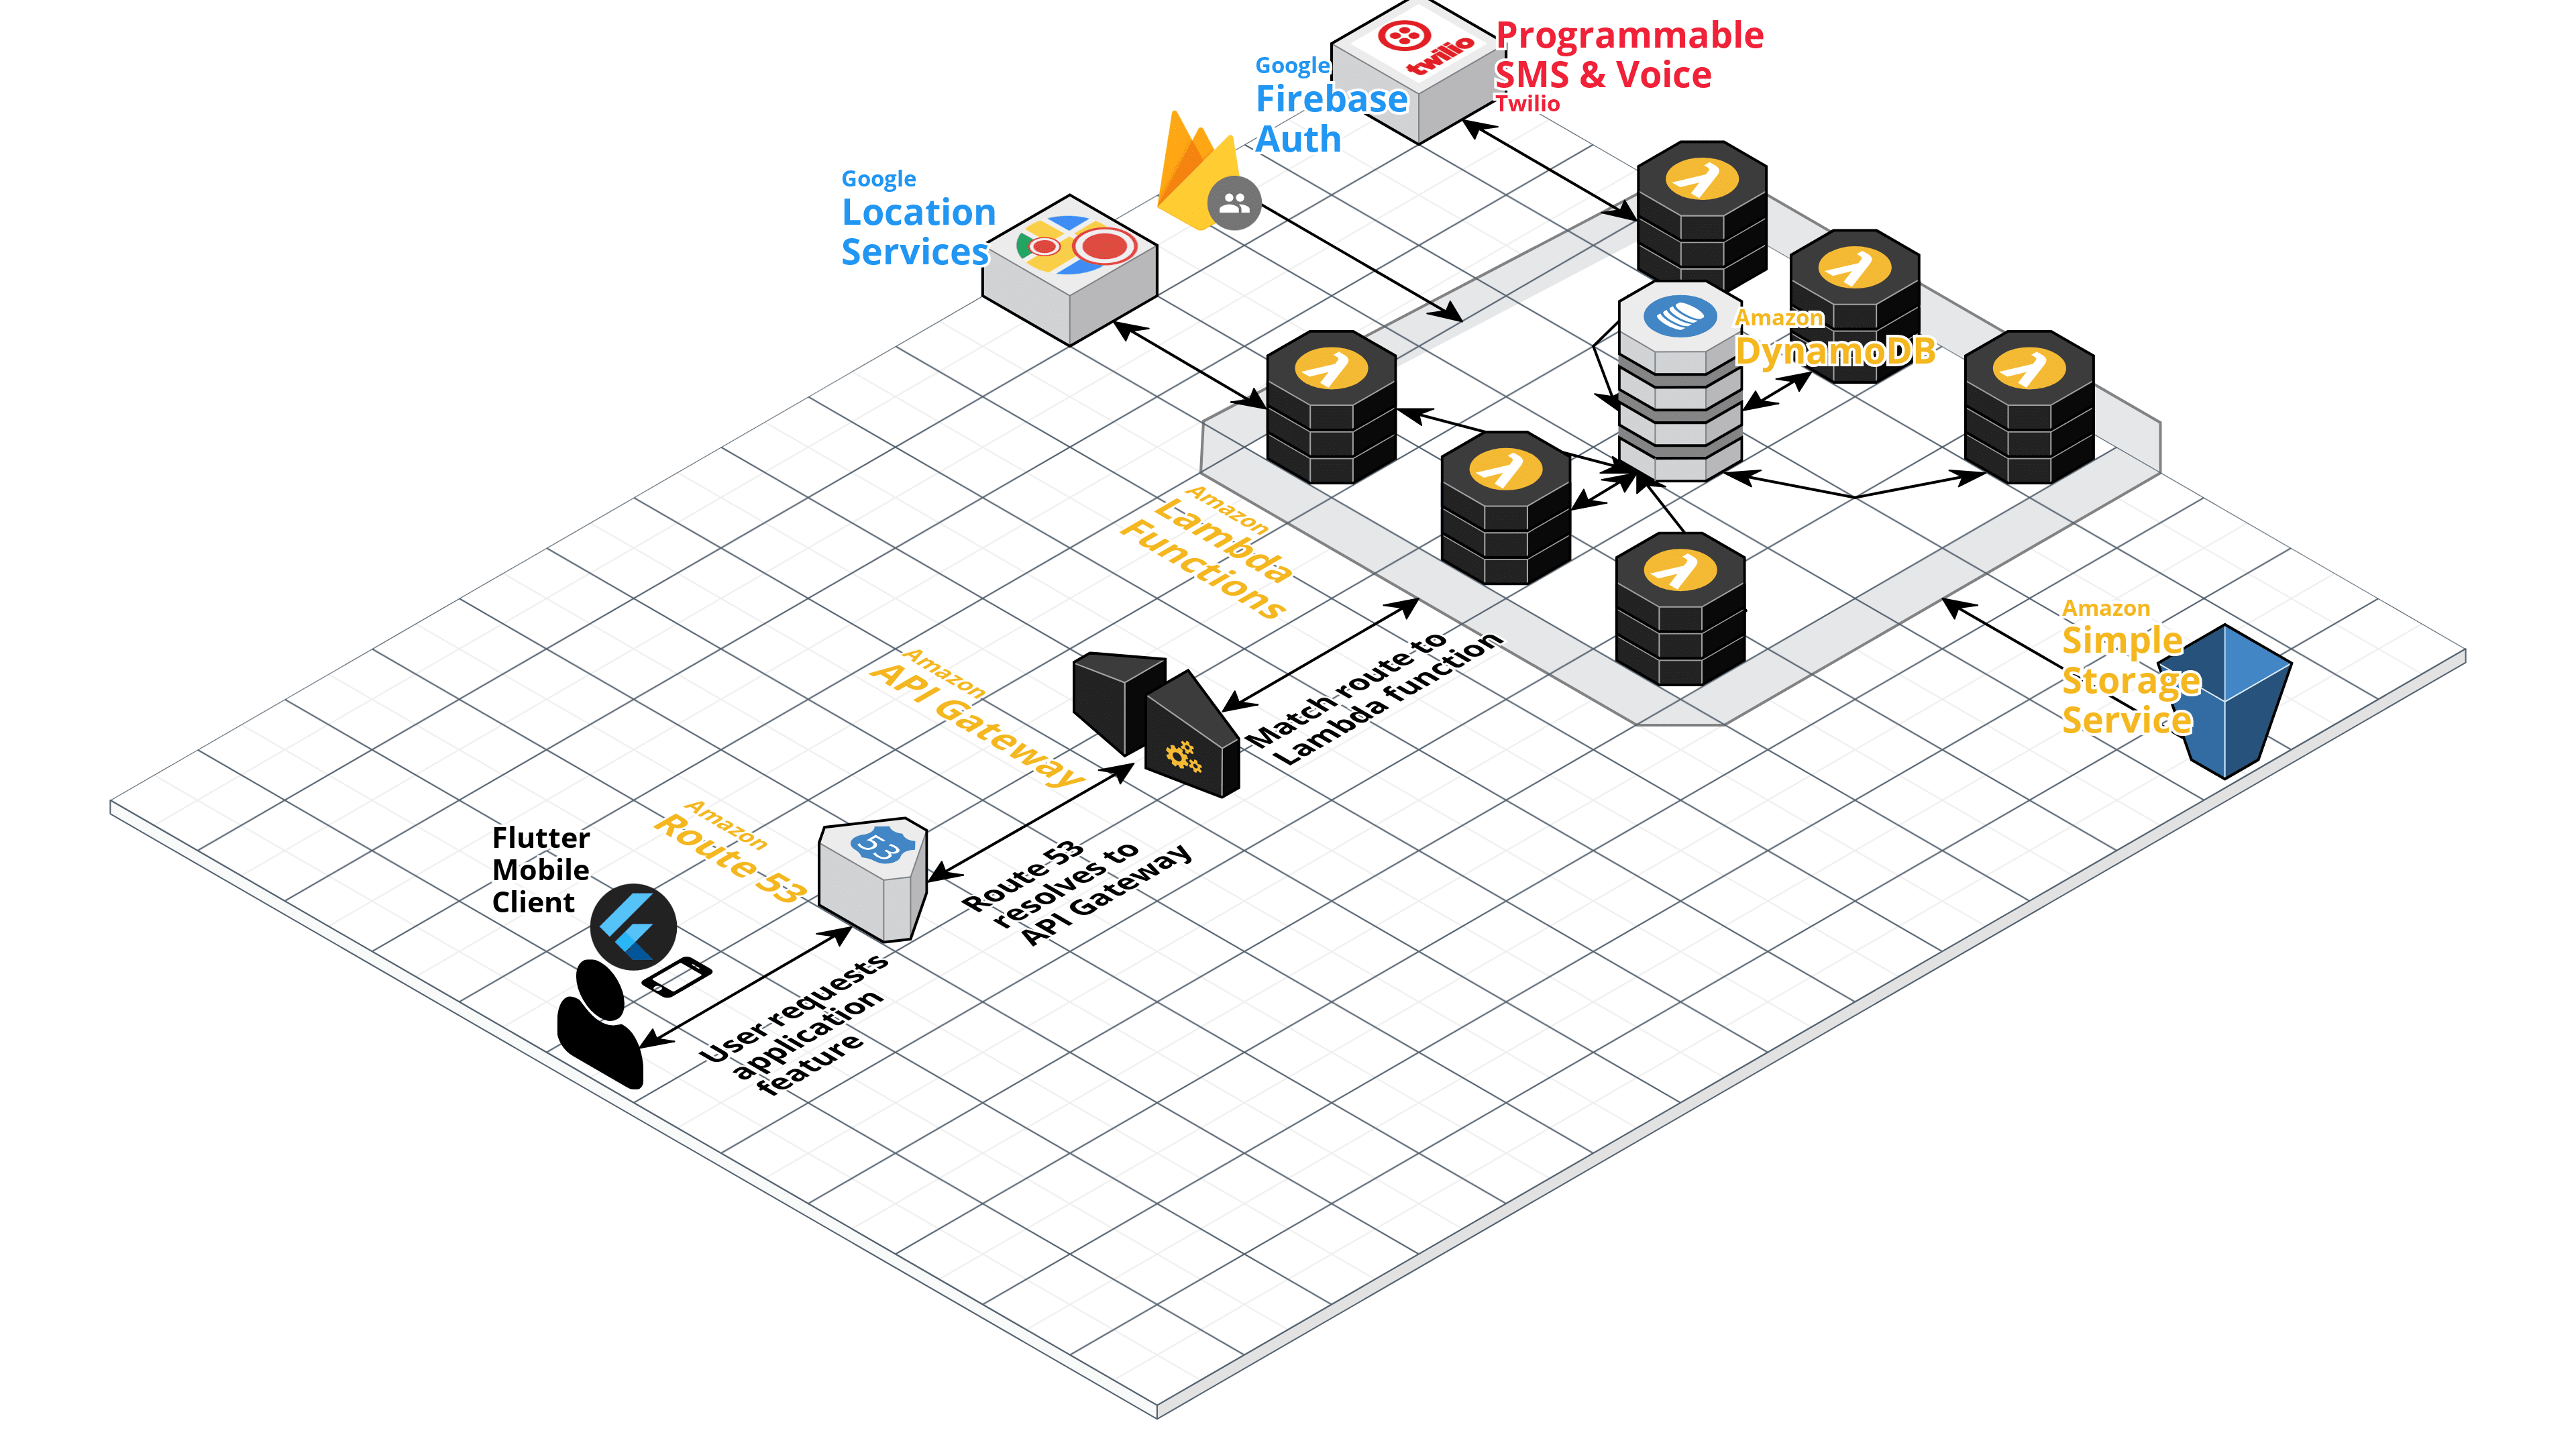
\includegraphics[scale=.15]{EmergenSeek-Backend.PNG}
}
\caption{Cloudcraft \cite{one} diagram of the AWS resources and external APIs necessary for the backend.}
\label{fig:1}	
\end{center}	
\end{figure}
	
\begin{thebibliography}{9}
\bibitem{one}
Cloudcraft ~ \url{https://cloudcraft.co}

\end{thebibliography}
\end{document}

